\documentclass[11pt]{article}
\usepackage{amssymb,amsmath,amsthm,url,subfigure, multirow,hyperref}
\usepackage{graphicx}
\usepackage{color}
\usepackage{enumerate}

\usepackage{gensymb}

\begin{document}

\section{Plan}
At a high level the idea (was/is at this point/might be) is:
\begin{itemize}
\item Somehow get our hands on a model of all (most) middleboxes in the
network. This might be computed using program analysis or be provided by
someone etc.
\item Hook up middleboxes as a network, verify that some high level policies (for instance isolation) holds given the model. 
\item If step 2 reveals that things are peachy, generate some packets to verify that the model itself is actually behaving reasonably.
\item Prosper.
\end{itemize}

For now we (I) were focusing on step 2. In particular the plan was to generate models for a variety of middleboxes and
see what we could do with this. Since I was having a hard time actually doing the model generation (I did not know what
part of the model was relevant, amount of detail required, etc.), I decided to generate only two models and try and
actually prove something in a simple network.

For what follows, most of the proofs and such were generated using \href{http://z3.codeplex.com/}{Z3} a SMT solver from
MSR.

\section{Models}
\begin{itemize}
\item Firewall: A really simple firewall that just does packet filtering, i.e. it just accepts or denies based on packet
source and destination addresses. (I have
included actual models at the end of the document, however they are long and not necessarily interesting to read. 

\item Web Proxy: Vyas's SIGCOMM paper pointed out that webproxies were a pretty reasonable example of a middlebox which
changed packet headers enough to make it hard to correlate input and output. This seemed exactly like something that
would trigger a case where the firewall would make a bad decision, so I ended up modeling a web proxy.

Actually the webproxy modeled is somewhat boring, when a packet is received it currently just changes the packet source
(to its own address) and sends it on. I also have a version where it can either generate this new packet or return a
cached response but I haven't set up a network where this behavior would make sense yet, more on this later.

Also webproxies like Squid include firewalls, so in some sense both these models are really in combination only
modeling one middlebox.
\end{itemize}

Both of these models are general (one could change the firewall rules trivially), which I think is useful.

In general setting up the models is hard, largely because they need to be exhaustively specified, for instance one of
the logical statements in the firewall states that if a firewall sends a packet $p$ it must have received the packet
$p$.
This might seem applicable to every element, but it in fact isn't applicable to the webproxy, where instead the logical
rule is that if the proxy sends a packet $p$ it must have received a packet $p'$ which has the same destination and
looks similar (more on similarity) in a second. The fear here is that at the end of this we might accidentally end up
taking 362 pages proving $1 + 1 = 2$.

Also, I am not entirely sure I have not over or underconstrained any of the models.

\section{General Network Model}
The other concern has been what information should the network track. Currently the model of a packet contains the
source, destination and origin (which is what overall policy predicates are based on). However the information contained
in a packet and rules for the network seem to be dependent on both the middleboxes being modeled and the overall policies being
tested (for instance if the policies were predicated on packet content then one would need to model the contents of the
packet). I am afraid about how general this might be.

\section{Results so Far}
\begin{figure*}[!h]
\begin{center}
\subfigure[Firewall then Web Proxy]{
    \centering
    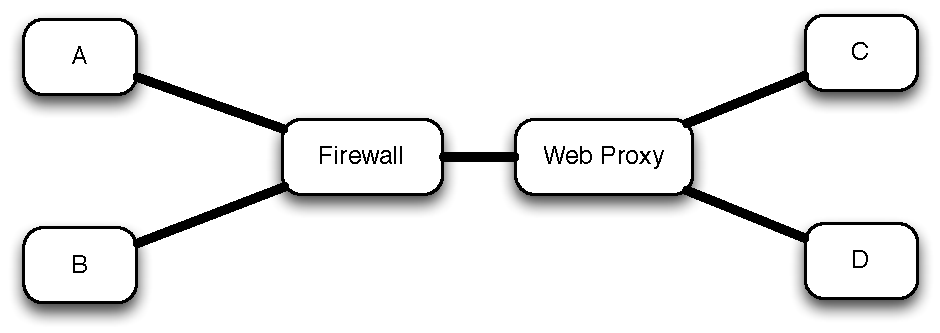
\includegraphics[width=0.47\textwidth]{./firewallwebproxy.pdf}
    \label{fig:fwwp}
}
\subfigure[Webproxy then Firewall]{
    \centering
    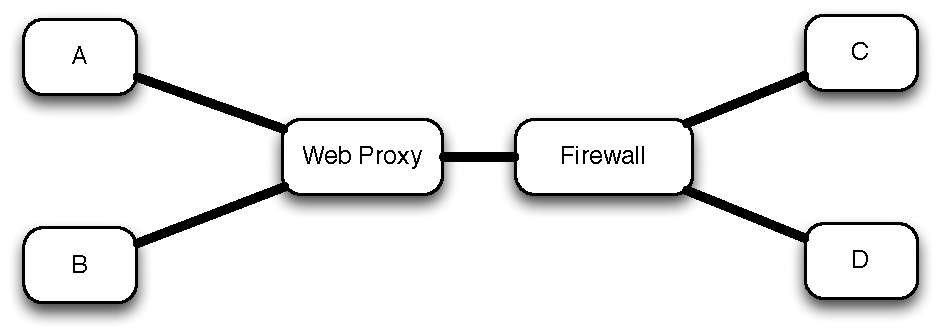
\includegraphics[width=0.47\textwidth]{./webproxyfirewall.pdf}
    \label{fig:wpfw}
}
\caption{Two topologies}
\label{fig:topologies}
\end{center}
\end{figure*}
Consider the two topologies in Figure~\ref{fig:topologies} and Firewall rules that disallow communication between
endhosts $A, C$ and $B, D$. Globally we want to ensure that $B$ cannot ever induce a packet to be sent to $D$ and $A$
cannot ever induce a packet to be sent to $C$. This policy is only enforceable in Figure~\ref{fig:fwwp} since the packet
looses information that is required for enforcement when it goes through the web proxy.

Currently we can generate counter examples for Figure~\ref{fig:wpfw} where the global policy does
not hold. Similarly for Figure~\ref{fig:fwwp} it can prove that the global policy does hold (by showing that no packets
satisfy the negation of the global constraints).

The problem here is that that first-order logic with quantifiers ($\forall$ and $\exists$) is
undecidable and will sometimes trip up the solver. Normally one tries to reexpress the constraints or add additional
(redundant) constraints for the solver to work, but I haven't yet figured out what combination of constraints will help.

 I am also trying to think through a way of expressing all of this logic that does not
involve these quantifiers but I don't know if that is doable. Figuring out what to do with unknowns might be a useful
thing to do.

\section{Other Concerns}
This is generally a problem for this sort of thing, but on average proof that there is a bug can be gotten really
quickly, but proving that there is no bug can take quite long. So for instance the case in Figure~\ref{fig:fwwp} takes
several minutes to run on a VM running on my laptop. Partly this is since disproving the existence of a packet can
require exploring the entire space. 
\section{The Models}
This is boring, I had to write this to reason about my code and it seemed like it might be useful someday.
\subsection{Network}
\textbf{Sets:}
\begin{align*}
Endhost &= \{A, B, C, D, Firewall, Proxy\}\\
Address &= set\ of\ addresses\\
Packet  &= [(src, dest, origin) src\in Address, dest\in Address, origin\in Endhost]
\end{align*}

\textbf{Functions:}
\begin{align*}
hostHasAddr &: Endhost\times Address \rightarrow bool\ \text{[A host can have several addresses]}\\
addrToHost  &: Address \rightarrow Endhost\ \text{[Address for host]}\\
send        &: Endhost\ (src) \times Endhost\ (dest) \times Packet \rightarrow bool\\ &\text{[True indicates a packet was
sent from source to destination]}\\
recv        &: Endhost\ (src) \times Endhost\ (dest) \times Packet \rightarrow bool\\ &\text{[True indicates a packet
was received at the destination from source]}
\end{align*}

\textbf{Constraints}
\begin{gather*}
\forall eh\in Endhost, ad\in Address\ hostHasAddr(eh, ad) \iff addrToHost(ad) = eh\\
\forall eh\ \exists ad\ hostHasAddr(eh, ad)\ \text{[All hosts are addressable]}\\
\forall e1,e2\in Endhost, p\in Packet\ recv(e1,e2,p) \iff send(e1,e2,p)\ \text{[No losses, no phantom packets]}\\
\forall e1,e2,\ p\ recv(e1,e2,p) \Rightarrow \exists e3\ send(addrToHost(p.src), e3, p)\\
\text{[No spoofing of sources]}\\
\forall e1,e2,\ p\ recv(e1,e2,p)\Rightarrow e1 \neq e2\text{[No loopback]}
\end{gather*}

\subsection{Endhost}
Presented here for endhost $A$ (same thing applies to $B, C, D$, but not to $Firewall$ and $Proxy$). This is for the
case where $A$ is connected to the Firewall (i.e. Figure~\ref{fig:fwwp}). Also the first two constraints come from $A$
having only one network address.
\begin{gather*}
\exists addr_a\in Address\ addrToHost(addr_a) = A\\
\forall a\in Address\ addrToHost(a) = A \Rightarrow a = addr_a\\
\forall eh, p\ recv(eh, A, p) \Rightarrow hostHasAddr(A, p.dest)\\
\forall eh, p\ send(A, eh, p) \Rightarrow hostHasAddr(A, p.src)\\
\forall eh, p\ send(A, eh, p) \Rightarrow p.origin = A\\
\forall eh, p\ send(A, eh, p) \Rightarrow eh = Firewall\\
\forall eh, p\ recv(eh, A, p) \Rightarrow eh = Firewall\\
\end{gather*}

\subsection{Firewall}
Rules here are $A$ cannot communicate with $C$, and $B$ cannot communicate with $D$.
\begin{gather*}
\forall e1, p\ send(FW, e1, p)\Rightarrow \exists e2\ recv(e2, FW, p)\\
\forall eh, p\ recv(eh, FW, p)\Rightarrow eh = A \lor eh = B \lor eh = proxy\\
\forall eh, p\ send(FW, eh, p)\Rightarrow eh = A \lor eh = B \lor eh = proxy\\
\forall eh, p\ send(FW, eh, p)\Rightarrow \neg((p.src = A \land p.dest = B) \lor\ldots)\\
\end{gather*}

\subsection{Proxy}
\begin{gather*}
\forall eh, p\ recv(eh, PROXY, p)\Rightarrow eh = C \lor eh = D \lor eh = FW\\
\forall eh, p\ send(PROXY, eh, p)\Rightarrow eh = C \lor eh = D \lor eh = FW\\
\forall eh, p\ send(PROXY, eh, p)\Rightarrow hostHasAddr(PROXY, p.src)\\
\forall e1, p\ send(PROXY, eh, p)\Rightarrow \exists e2, p2\ recv(e2, PROXY, p2) \land\\
\ \ \ \ \ \ \ \ p2.origin == p.origin\land p2.dest== p.dest\land hostHasAddr(p.origin, p.src)\\
\end{gather*}
\end{document}
